\chapter{B Tagging Studies}
\label{c:b_tagging_studies}

In order to study \ttbar events, event selections often use the reconstruction of jets as a key part of the
event signature. More specifically, b tagging is used to identify those jets which come from a b quark. There
are several algorithms which carry out b tagging in CMS: Combined Secondary Vertex, CombinedSecondaryVertex,
CombinedSecondaryVetexMVA, JetBProbability, JetProbability, SimpleSecondaryVertex (High Efficiency),
SimpleSecondaryVertex (High Purity), SoftMuon, SoftMuonByPt, SoftMuonByIP3d, TrackCounting (High Efficiency),
TrackCounting (High Purity). These algorithms perform analyses on the jet in question and produce a
discriminator output (simply a number). In all cases, a more positive discriminator value indicates a jet that
is more likely to be a b flavour jet. The performance of the different algorithms vary depending on which jet
characteristics are used to calculate the discriminator.

The curent CMS recommendation is to use the Combined Secondary Vertex for physics analyses. This algorithm
reconstructs the event vertices using the Trimmed Kalman Vertex Finder TODO:DESCRIBE THIS?
%TODO: MORE INFO ABOUT THIS, SEE PRESENTATION
and applies cuts to these vertices in order to find a secondary vertex, the b decay vertex.
Depending on how many candidate secondary vertices are found, different combinations of variables such as
impact parameter, flight distance significance between primary and secondary vertices, kinematics and
secondary, kinematics and secondary vertex information are used to calculate a discriminator value \cite{CSV}.

The JProbability algorithms take all tracks, calculate the signed impact parameter significance and calculate
the discriminator based on the negative log of the confidence level that all tracks are from the primary
vertex. The Simple Secondary Vertex uses an adaptive vertex finder to reconstruct the secondary vertex and
calculate the disciminator based on variables such as the decay length significance. The Soft Muon algorithms
use the detection of a muon from the semi-leptonic decay of a b quark and a neural net analysis. The Track
Counting algorithms simply take all the tracks within a jet and order them by decreasing order o signed impact
parameter significance, with the discriminator being the significance of the second track (high efficiency) or
the third track (high purity).

TODO: INCLUDE A MORE DETAILED DESCRIPTION OF EACH ALGORITHM? ALSO INCLUDE PLOTS FOR OTHER ALGORITHMS?
%TODO: INCLUDE A MORE DETAILED DESCRIPTION OF EACH ALGORITHM?

Analysing a Fall 2011 \ttbar Madgraph Monte Carlo sample (/TTJets\_TuneZ2\_7TeV-madgraph-tauola/) simulated in
CMSSSW 44X, all algorithms produced higher discriminator values for the b jets in the sample than the light
jets (up, down and strange flavour), gluon jets and c flavour jets. All histograms were normalised to unity in
order to facilitate shape comparison. Figure~\ref{fig:CSV_discriminators} shows these normalised histograms
produced by the CSV algorithm.

\begin{figure}[hbtp]
   \centering
     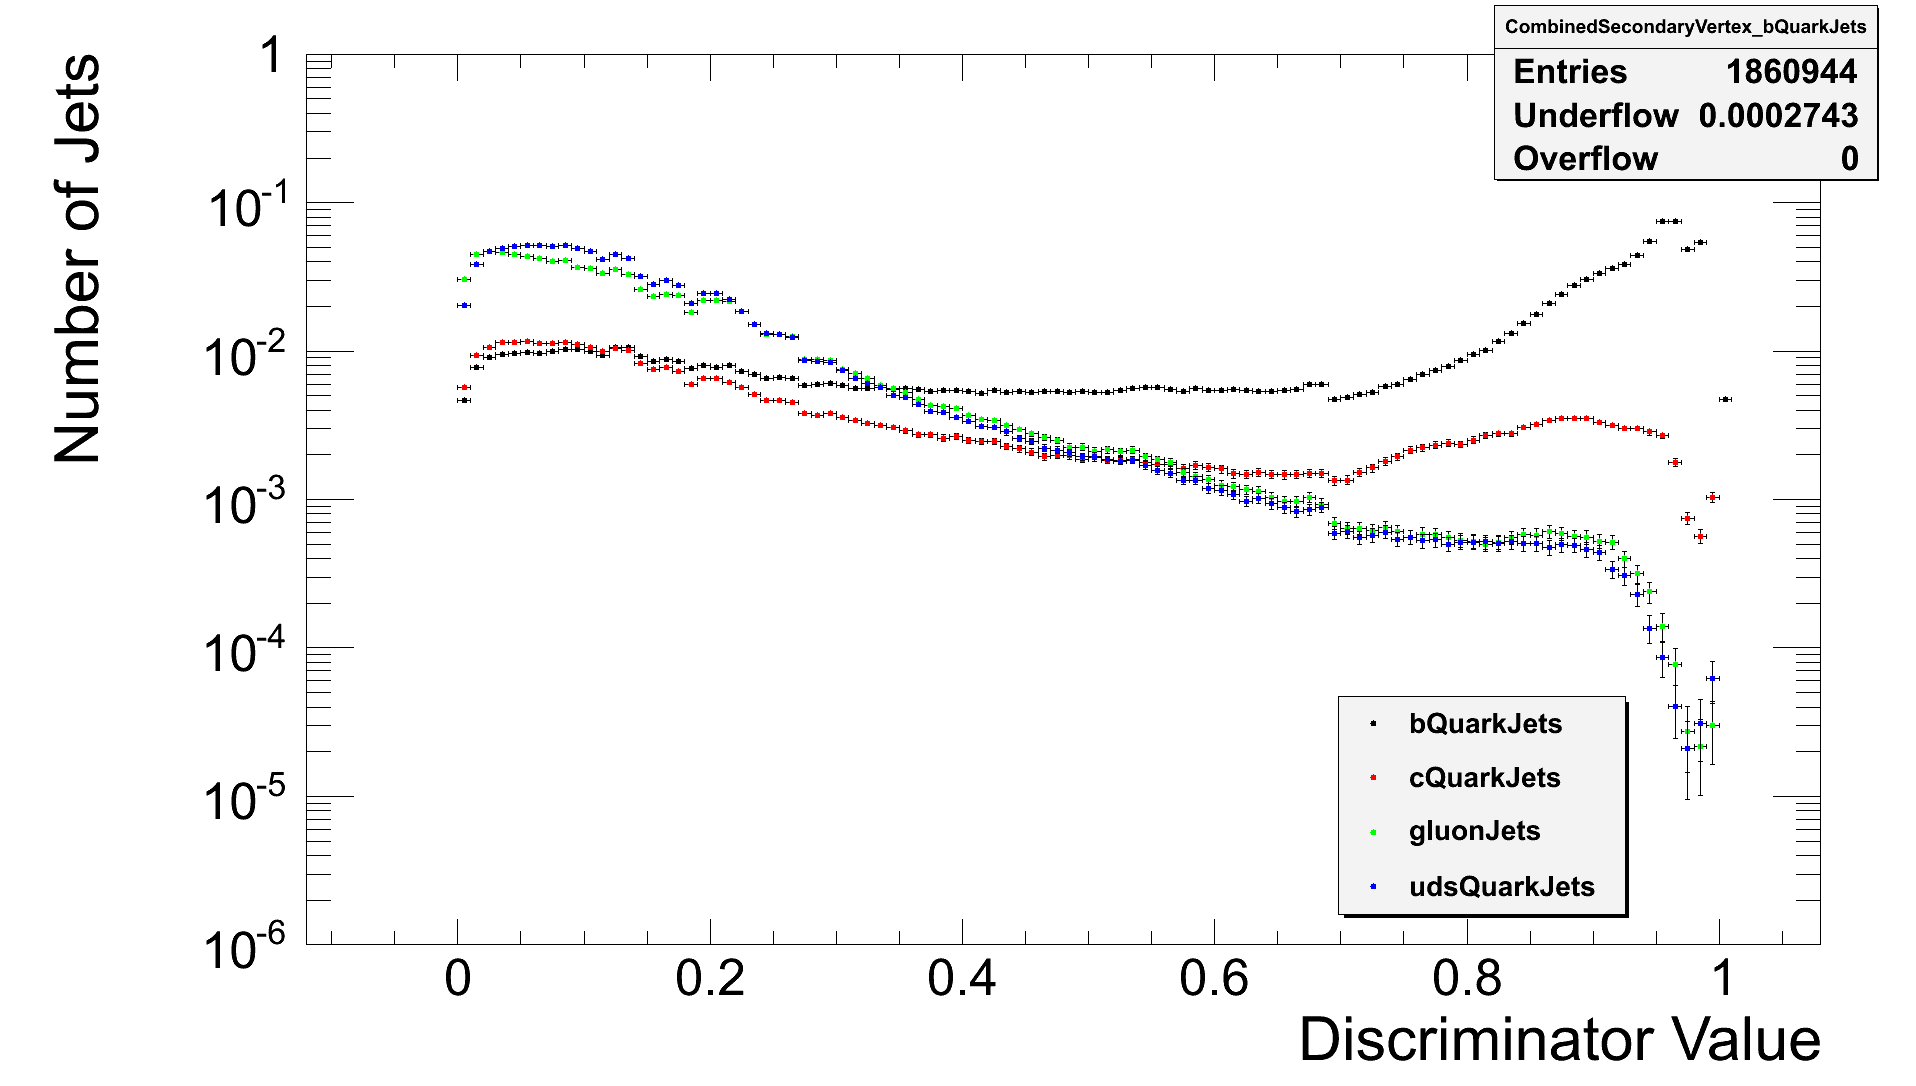
\includegraphics[width=\textwidth]{Chapters/04_Analysis/04a_BTags/Images/CombinedSecondaryVertex_discriminator_combined}\\
     \caption{Discriminator values produced by the Combined Secondary Vertex algorithm for all 4 jet flavours after normalisation}
     \label{fig:CSV_discriminators}
\end{figure}

\section{Efficiency}
\label{s:efficiency}

Cutting on a desired discriminator value allows the efficiency of that cut value to be found by taking the
area of the histogram to the right of the cut value, as a proportion of the total histogram area. Cuts were
made through the whole range of discriminator values in order to create plots of b tag efficiency as a
function of cut value. In practice, the aim is to acheive a high efficiency for b jets and a low efficiency
for all other jet flavours. Figure~\ref{fig:jet_efficiencies} shows how the efficiency for light, gluon and c
jets vary as a function of b jet efficiency for cuts made on the CSV discriminator.

\begin{figure}[hbtp]
   \centering
     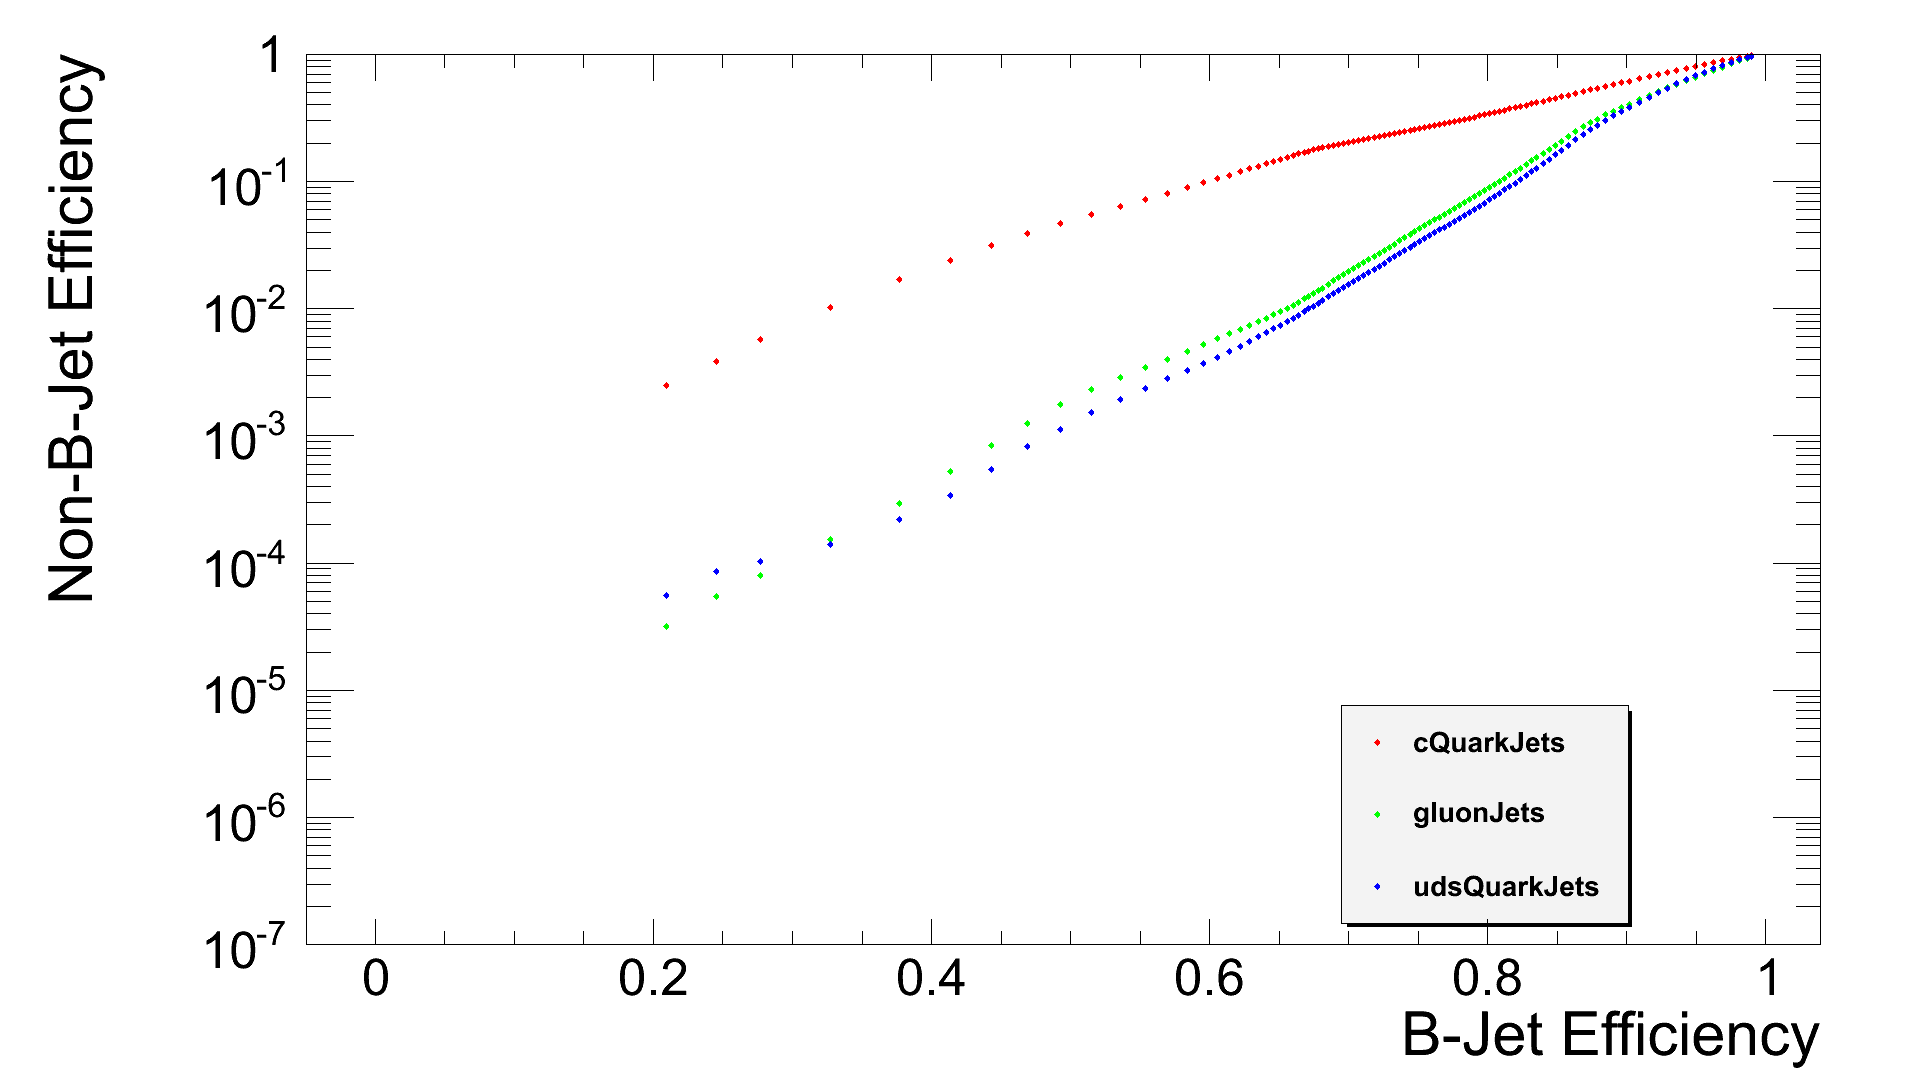
\includegraphics[width=\textwidth]{Chapters/04_Analysis/04a_BTags/Images/CombinedSecondaryVertex_nonBJetEfficiency_v_BJetEfficiency}\\
     \caption{Non b jet effiencies as a function of b jet efficiency for the CSV algorithm}
     \label{fig:jet_efficiencies}
\end{figure}

\section{Algorithm Comparison}
\label{algorithm_comparison}

The performances of the various algorithms can be compared in Figure~\ref{fig:uds_eff_v_b_eff}.

\begin{figure}[hbtp]
   \centering
     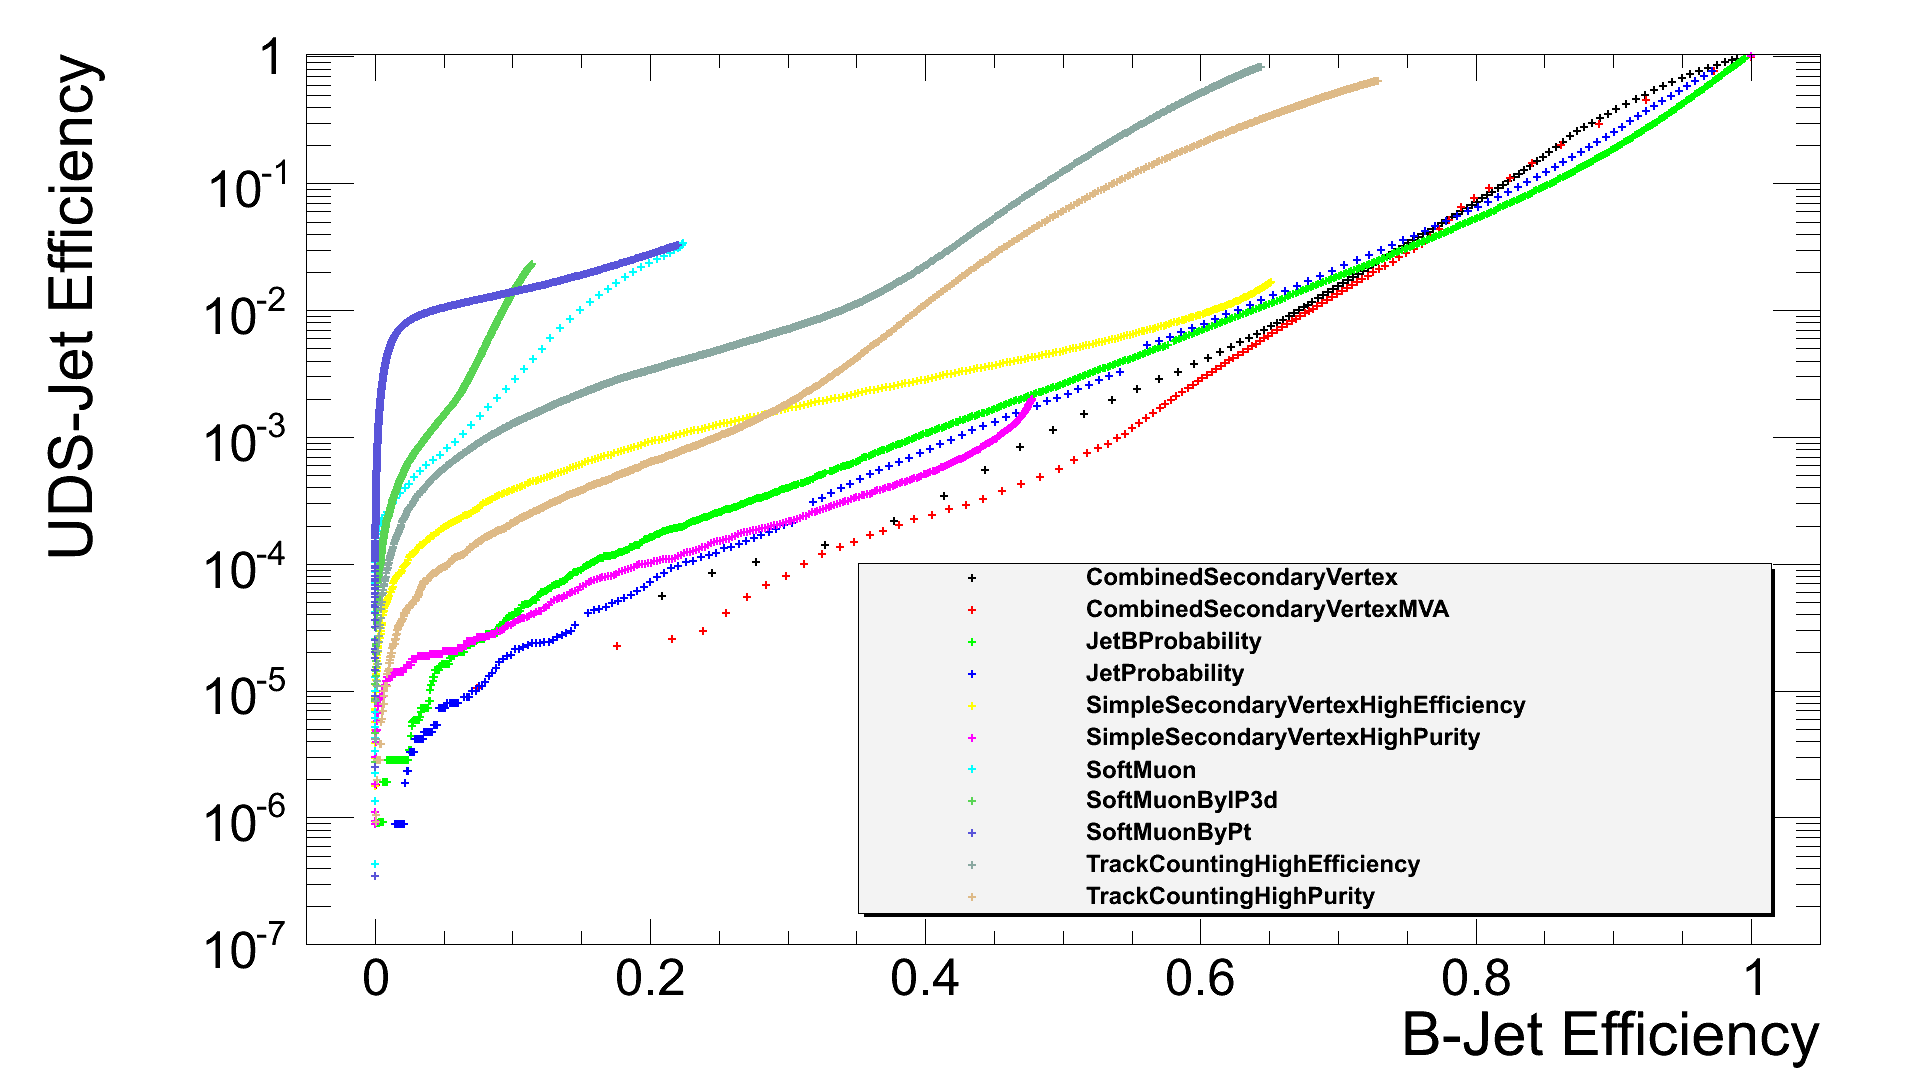
\includegraphics[width=\textwidth]{Chapters/04_Analysis/04a_BTags/Images/UDS-JetEfficiency_v_B-JetEfficiency_withLegend}\\
     \caption{UDS jet efficiencies as a function of b jet efficiencies for all algorithms}
     \label{fig:uds_eff_v_b_eff}
\end{figure}

Algorithms which reach closest to the lower lower right of the plot show better performance, according to the
requirements of high b jet efficiency and low light jet efficiency. It can be seen that not all algorithms
reach 100\% efficiency for b jets due to some being inherently limited by their methods EXPAND ON THIS. For
instance, the soft muon algorithms all show low maximum b jet efficiencies due to the low b hadron semi
leptonic branching ratio to muon of approximately 11\% (or 20\% when further decays are included)
\cite{btagging_in_CMS}. The 2011 and 2012 CMS recommended b tagger is the Combined Secondary Vertex with
operating point cuts of 0.244 (loose), 0.679 (medium) and 0.898 (tight) corresponding to 10\%, 1\% and 0.1\%
light jet and gluon jet efficiencies respectively. These cuts are indicated by the horizontal lines on
Figure~\ref{fig:uds_eff_v_b_eff}. It can be seen that for the tight and medium cuts, the CSV MVA algorithms
provides highest b jet efficiency and lowest light jet efficiency, followed closely by the CSV algorithm. At
approximately 3\% light jet efficiency, there is a convergence of many b taggers which all provide similar
performance, above which the JetBProbability algorithm gives marginally highger b jet efficiency.

